\documentclass[final,xcolor=table,svgnames]{beamer}
\usepackage[english]{babel}
\usepackage[T1]{fontenc}
\usepackage{graphicx}
\usepackage{hyperref}
\usepackage{url}
\usepackage{tikz}
\usepackage{doi}
\usepackage{fontawesome}
\usepackage{academicons}
\usepackage{fontspec}
\usepackage{textpos}
\usepackage{listings}
\usepackage{bbding}


% Fonts
% -------------

\usepackage{array}
\newcolumntype{L}[1]{>{\raggedright\let\newline\\\arraybackslash\hspace{0pt}}m{#1}}
\newcolumntype{C}[1]{>{\centering\let\newline\\\arraybackslash\hspace{0pt}}m{#1}}
\newcolumntype{R}[1]{>{\raggedleft\let\newline\\\arraybackslash\hspace{0pt}}m{#1}}

%\setmainfont{Arial}
\newcommand{\logoheight}{1cm}
\newcommand{\yestab}{{\cellcolor{LightGreen} Yes}}

\DeclareGraphicsExtensions{.pdf,.png,.PNG,.JPG,.jpg,.jpeg,.gif}
\graphicspath{
{./figures/},
{/home/ctroupin/Presentations/figures4presentations/logo/},
}


\setbeamertemplate{navigation symbols}{}
\setbeamertemplate{items}[square] 

\usefonttheme{professionalfonts} % using non standard fonts for beamer

\usetikzlibrary{arrows,shapes,backgrounds,spy,calc}
\tikzstyle{every picture}+=[remember picture]
\tikzstyle{na} = [baseline=-.5ex]

\definecolor{bluegher}{HTML}{4E519F}
\definecolor{mygrey}{rgb}{0.25,.25,.25}
\definecolor{commentcolor}{rgb}{0.75,.75,.75}
\definecolor{arrowcolor}{rgb}{0.1,0.1,0.1}
\definecolor{shadecolor}{rgb}{0.1,0.1,0.1}
\definecolor{bluesdn}{HTML}{0551A0}
\definecolor{darkbluesdn}{HTML}{044F9C}
\definecolor{bluetwitter}{HTML}{1DA1F3}

\definecolor{alertbg}{HTML}{FEFFBA}

\setbeamercovered{invisible}
\setbeamertemplate{items}[triangle] 

\newenvironment{boxalertenv}{\begin{altenv}%
      {\usebeamertemplate{alerted text begin}\usebeamercolor[fg]{alerted text}\usebeamerfont{alerted text}\colorbox{bg}}
      {\usebeamertemplate{alerted text end}}{\color{.}}{}}{\end{altenv}}

\newcommand<>{\boxalert}[1]{{%
  \begin{boxalertenv}#2{#1}\end{boxalertenv}%
}}

\setbeamercolor{author}{fg=bluesdn}
\setbeamercolor{title}{fg=bluesdn,bg=red}
\setbeamercolor{institute}{fg=bluesdn}
\setbeamercolor{frametitle}{fg=bluesdn,bg=white}
\setbeamercolor{item projected}{fg=black}

\setbeamerfont{sectiontitle1}{size=\huge,family=\rmfamily}
\setbeamerfont{sectiontitle2}{size=\fontsize{40}{20}\selectfont,shape=\itshape,family=\rmfamily}
\setbeamerfont{author}{size=\large}
\setbeamerfont{institute}{size=\normalsize}
\setbeamerfont{title}{size=\fontsize{34}{20}\selectfont,shape=\itshape,family=\rmfamily}
\setbeamerfont{subtitle}{size=\normalsize,family=\rmfamily}
\setbeamerfont{projected text}{size=\normalsize,family=\rmfamily}

\setbeamercolor{item projected}{bg=alertbg,fg=bluegher}

\setbeamertemplate{enumerate items}[square]
\setbeamertemplate{footline}[frame number]


\setbeamertemplate{frametitle}[default][left,leftskip=2.cm] % <-- choose here the leftskip you wish
\addtobeamertemplate{frametitle}{}{%
\begin{textblock*}{100mm}(0cm,-.9cm)
\includegraphics[height=1cm]{logo_seadatacloud_notransp.png}
\end{textblock*}}

\newcommand\mynum[1]{%
  \usebeamercolor{enumerate item}%
  \tikzset{beameritem/.style={circle,inner sep=0,minimum size=3ex,text=white,fill=bluesdn}}%
  \tikz[baseline=(n.base)]\node(n)[beameritem]{#1};%
}

%\setbeamersize{text margin left=1cm}

\newlength{\logoH}
\setlength{\logoH}{1cm}
\newcommand{\comment}[1]{\hfill\textcolor{commentcolor}{#1}}

\newcommand\Wider[2][3em]{%
\makebox[\linewidth][c]{%
  \begin{minipage}{\dimexpr\textwidth+#1\relax}
  \raggedright#2
  \end{minipage}%
  }%
}

%--------------------------------
\hypersetup{bookmarksopen=true,
bookmarksnumbered=true,  
pdffitwindow=true, 
pdfstartview=FitPage,
pdffitwindow=true,
pdftoolbar=true,
pdfmenubar=true,
pdfwindowui=true,
pdfsubject={SeaDataCloud, Data analysis, Interpolation, Diva, DIVAnd, EUDAT},
pdfauthor={C. Troupin, S. Watelet, A. Barth, J.M. Beckers},
bookmarksopenlevel=0,
colorlinks=true,
linkcolor=bluegher,anchorcolor=black,%
citecolor=bluegher,filecolor=black,%
menucolor=black,urlcolor=bluegher,%
pdfpageduration=1,%
}



\subtitle{"Putting the EOSC vision into practice"}
\title{DIVA software and the \faCloud}
\author[C.~Troupin]{{\faTwitter}~{\faAt}CharlesTroupin, A.~Barth, S.~Watelet \& J.-M.~Beckers}
\institute{University of Liège, GeoHydrodynamics and Environment Research}
\date{Porto (Portugal), 22-25 January, 2018}
\titlegraphic{\includegraphics[height=\logoheight]{logo_seadatacloud.png}
\includegraphics[height=\logoheight]{logo_uliege.jpeg}\includegraphics[height=\logoheight]{logo_gher}
}


\begin{document}
\thispagestyle{empty}  % to remove the page numbering
\newfontfamily\titletext{Carlito}

{
\usebackgroundtemplate{\includegraphics[width=\paperwidth]{seadatacloud_bg1.png}}
\begin{frame}
\begin{tikzpicture}[remember picture,overlay,every text node part/.style={align=center}]]
\node[yshift=-.5cm,text=bluesdn] at (current page.center) {\LARGE \titletext \inserttitle};
\node[yshift=-1.5cm,text=gray] at (current page.center) {\insertauthor};
\node[yshift=-2cm,text=bluesdn] at (current page.center) {\insertinstitute};

\node[yshift=1.5cm, xshift=-.5cm, text=bluesdn, anchor=east] at (current page.south east){\bf\scriptsize EUDAT Conference, Porto (Portugal), 22-25 January 2018}; 
%\node[yshift=1cm,xshift=-.5cm, text=bluesdn, anchor=east] at (current page.south east){\tiny sdn-userdesk@seadatanet.org - www.seadatanet.org}; 

\end{tikzpicture}
\end{frame}
}

\begin{frame}[b]
\frametitle{Can you guess the temperature at the "?"}

\Wider[2.cm]{
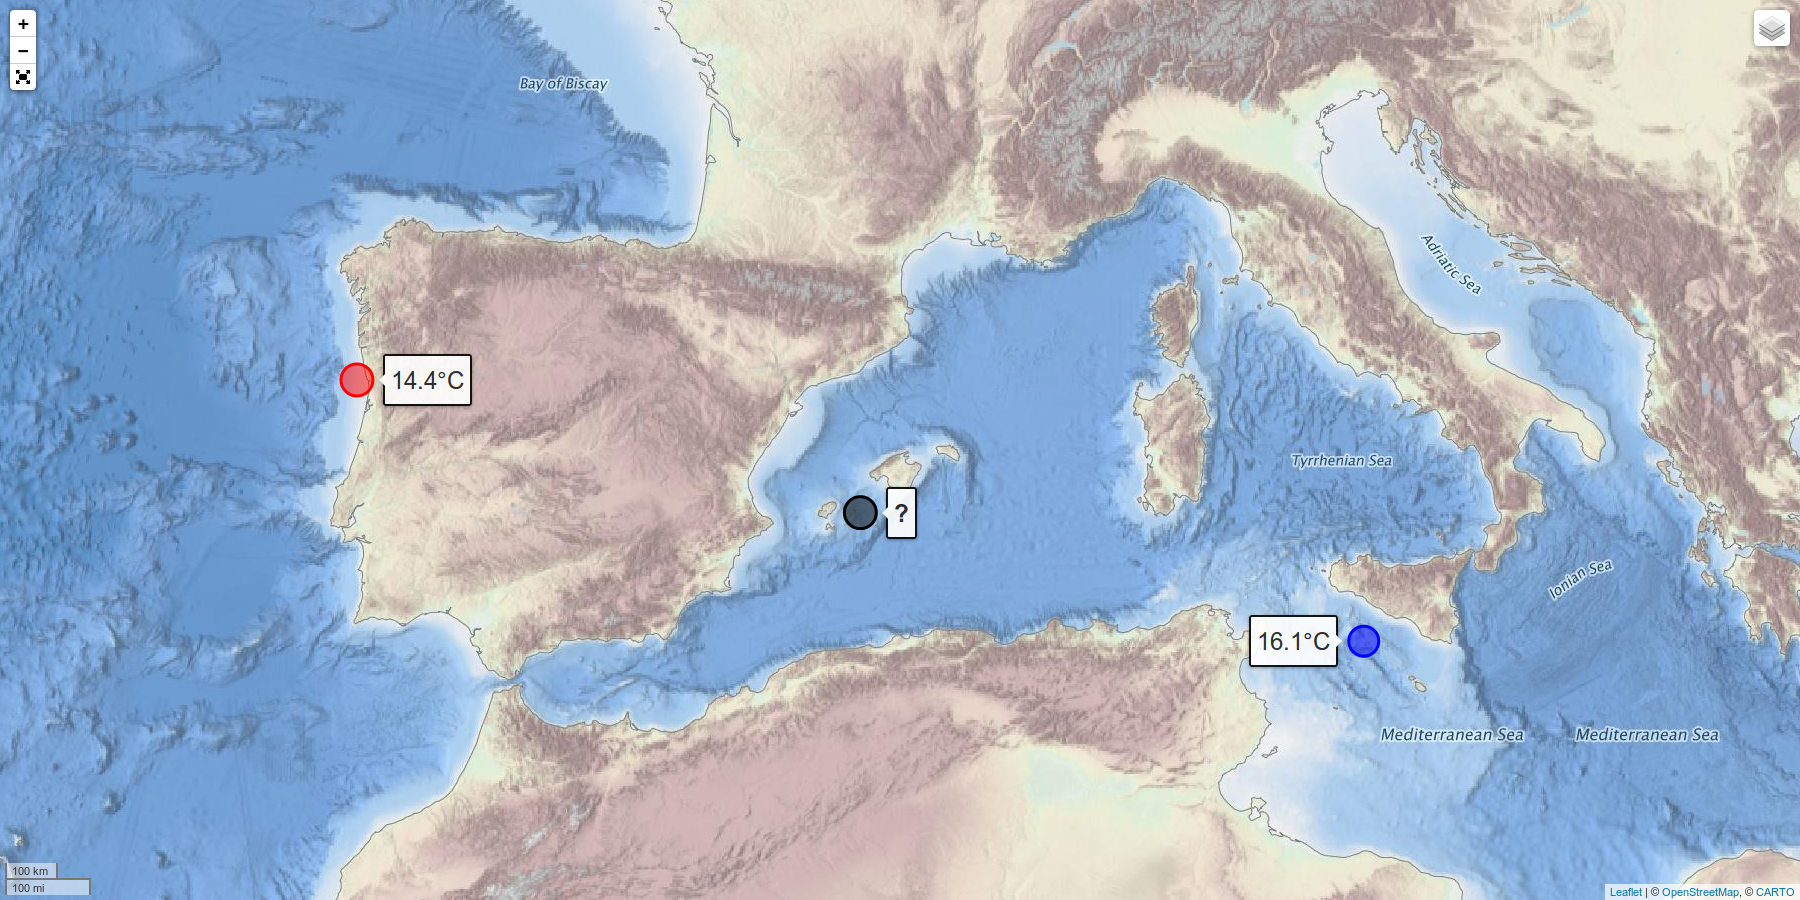
\includegraphics[width=\textwidth]{map_base.png}
}

\end{frame}

%----------------------------------------------------
\section{Spatial interpolation}
\subsection{Why is it needed?}
%----------------------------------------------------

\begin{frame}
\frametitle{~}

\fontsize{35}{20}\selectfont Spatial interpolation:\\Why is it needed?
\end{frame}

\begin{frame}[c]
\frametitle{Ocean observation is expensive and complex}

\onslide*<2>{
\centering
"\textit{A measurement not made is a measurement lost forever}"

\vspace{1cm}

"\textit{Collect once, use many times}" 
}

\onslide*<1>{
\includegraphics[width=\textwidth]{0_socib_obs}\\
{\tiny Credit: \url{www.socib.es}}
}

\end{frame}
%---------------------------------------------------------------------------------
\begin{frame}[b]
\frametitle{Can you guess the temperature at the "?"}

\onslide*<1-2>{$$\frac{14.4 + 16.1}{2} = 15.25^{\circ}\textrm{C}\qquad??$$}

\onslide*<1>{
\Wider[2.cm]{
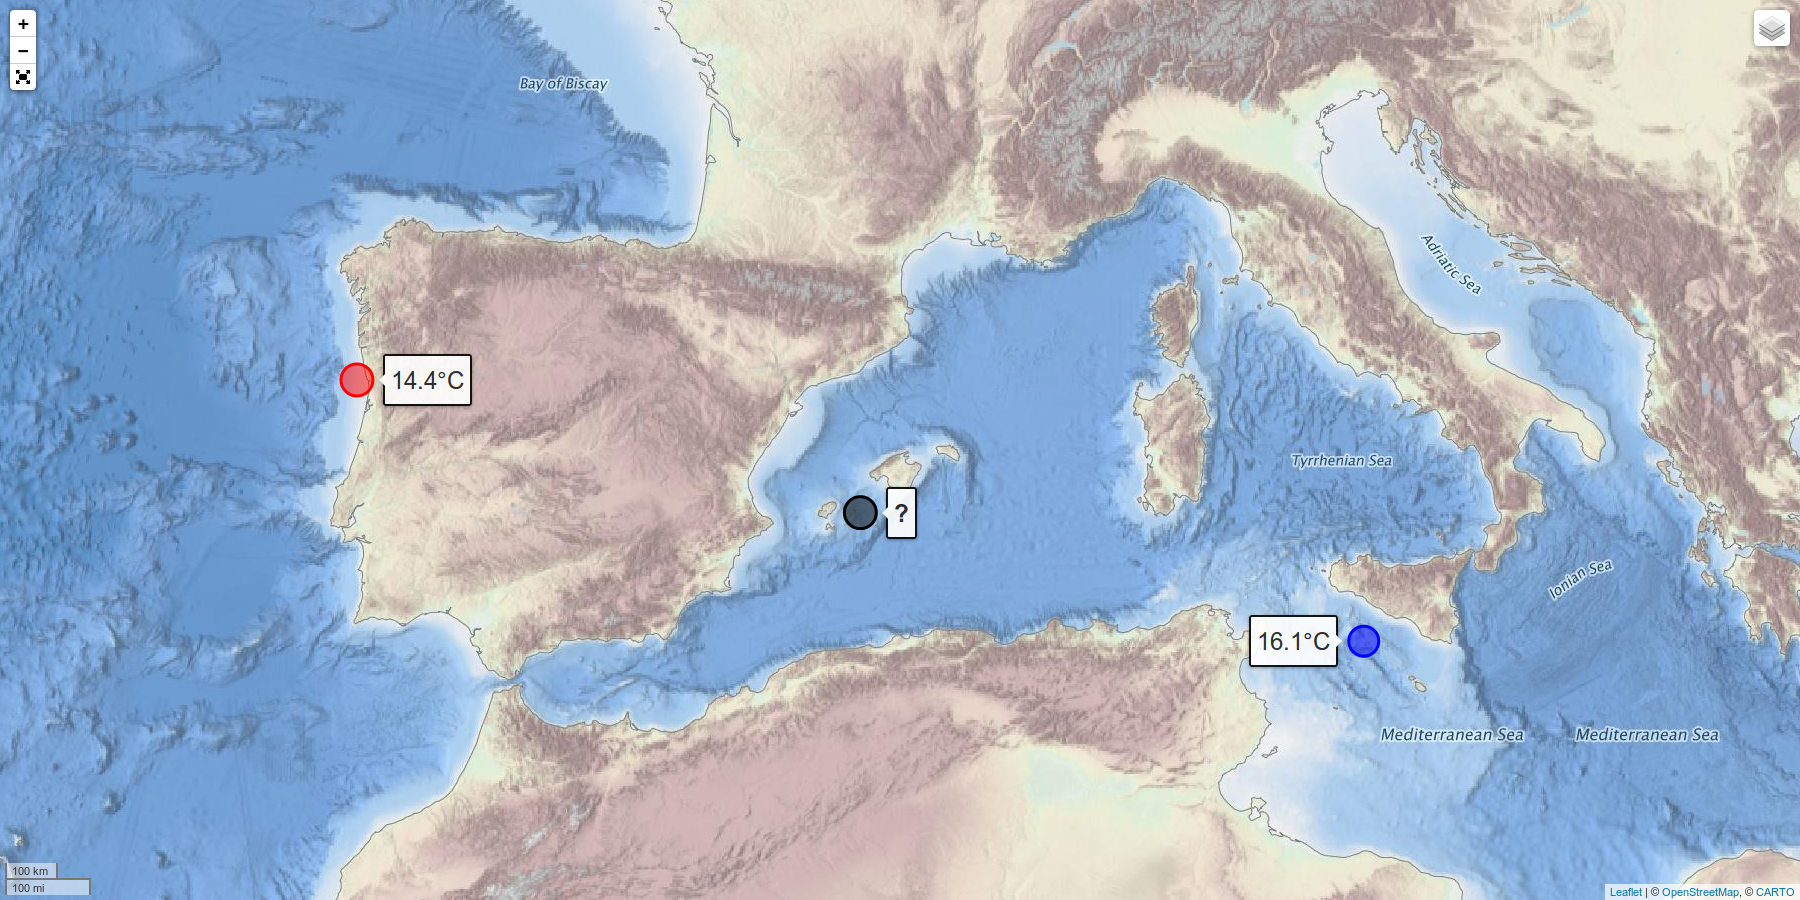
\includegraphics[width=\textwidth]{map_base.png}
}
}


\onslide*<2>{
\centering
\includegraphics[width=.4\textwidth]{notbad.jpg}
\vfill
~
}
\end{frame}

%---------------------------------------------------------------------------------
\subsection{Why is it not so easy?}

\begin{frame}
\frametitle{~}
6 reasons why\\ {\fontsize{35}{20}\selectfont spatial interpolation}\\ is not so easy
\end{frame}

%---------------------------------------------------------------------------------
\begin{frame}[b]
\frametitle{\mynum{1} Synopticity error}

Measurements not collected at the same time

\vspace{.5cm}

\Wider[2.cm]{
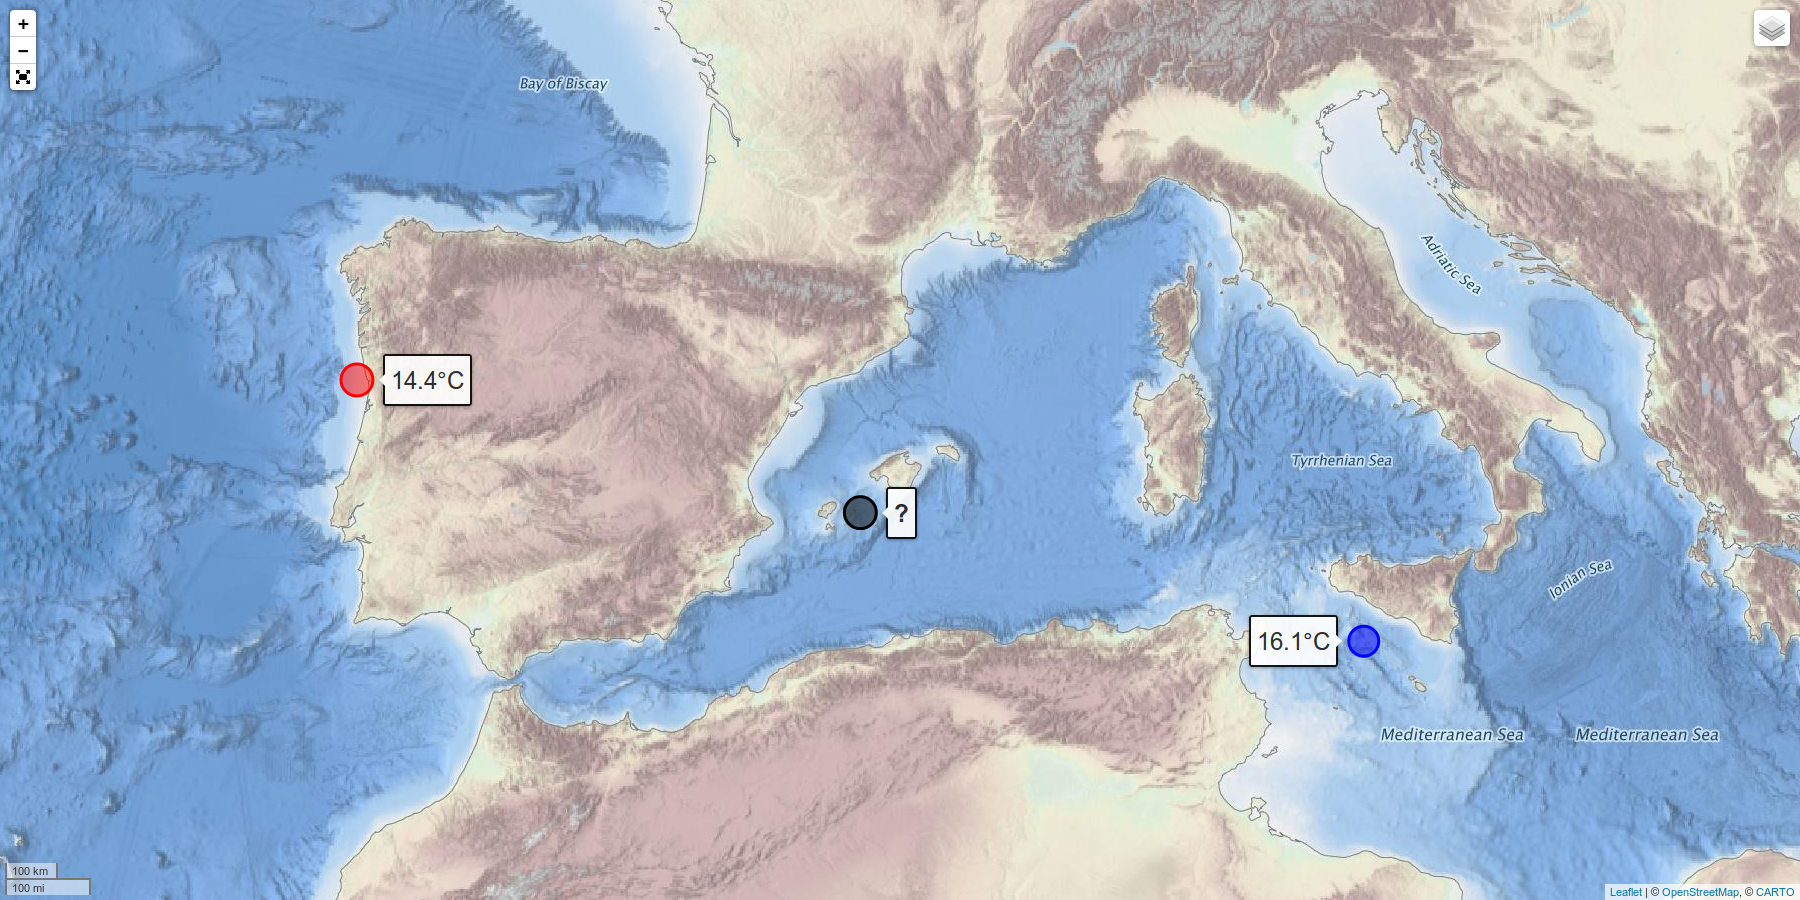
\includegraphics[width=\textwidth]{map_base.png}
}

\end{frame}

%---------------------------------------------------------------------------------
\begin{frame}[c]
\frametitle{\mynum{2} Representativeness error}

\Large{
What we measure is not always\\
what we intend to analyse
}

\vspace{2cm}

{\large\textbf{Example:} I want the mean annual temperature off Porto\\
but ships are only at sea when the weather is good}

\end{frame}

%---------------------------------------------------------------------------------

\begin{frame}[b]
\frametitle{\mynum{3} A lot of observations, but not everywhere}

\Wider[2.cm]{
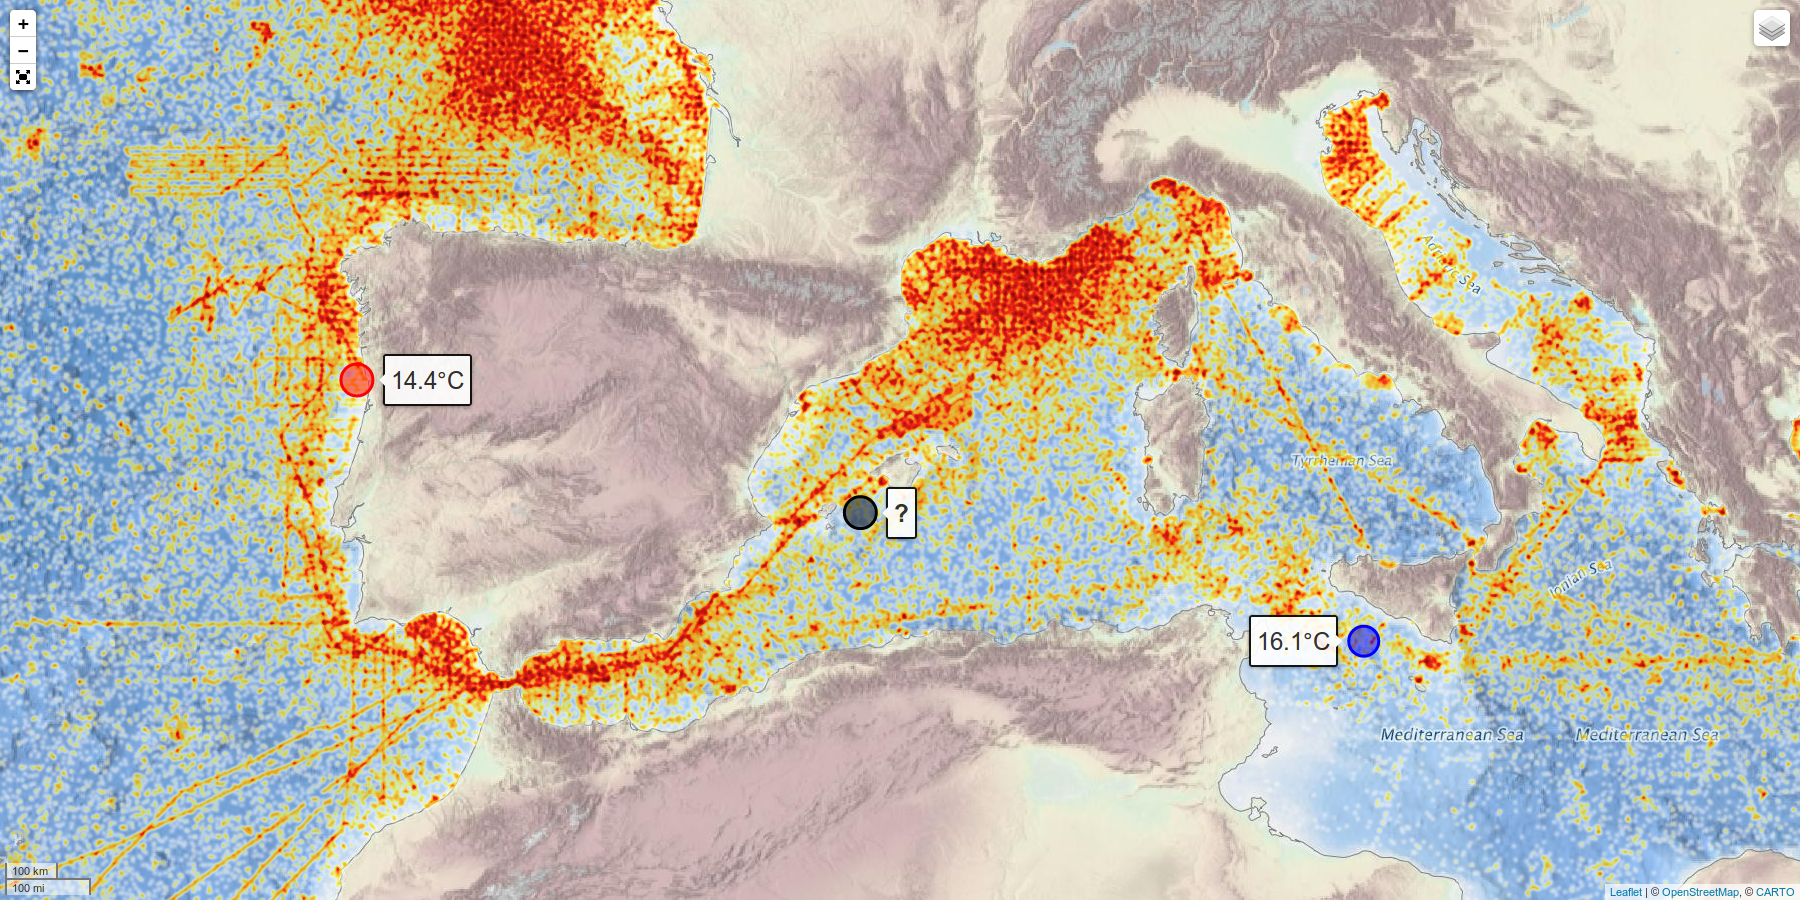
\includegraphics[width=\textwidth]{map_data.png}
}

\end{frame}

%---------------------------------------------------------------------------------
\begin{frame}[b]
\frametitle{\mynum{4} Need to interpolate at many locations}
\huge

\Wider[2.cm]{
\includegraphics<1>[width=\textwidth]{map_grid.png}
\includegraphics<2>[width=\textwidth]{map_finegrid.png}
}
\end{frame}

%---------------------------------------------------------------------------------
\begin{frame}[b]
\frametitle{\mynum{5} Anisotropy}

Land acts as a physical barrier\\


\vspace{.5cm}


\Wider[2.cm]{
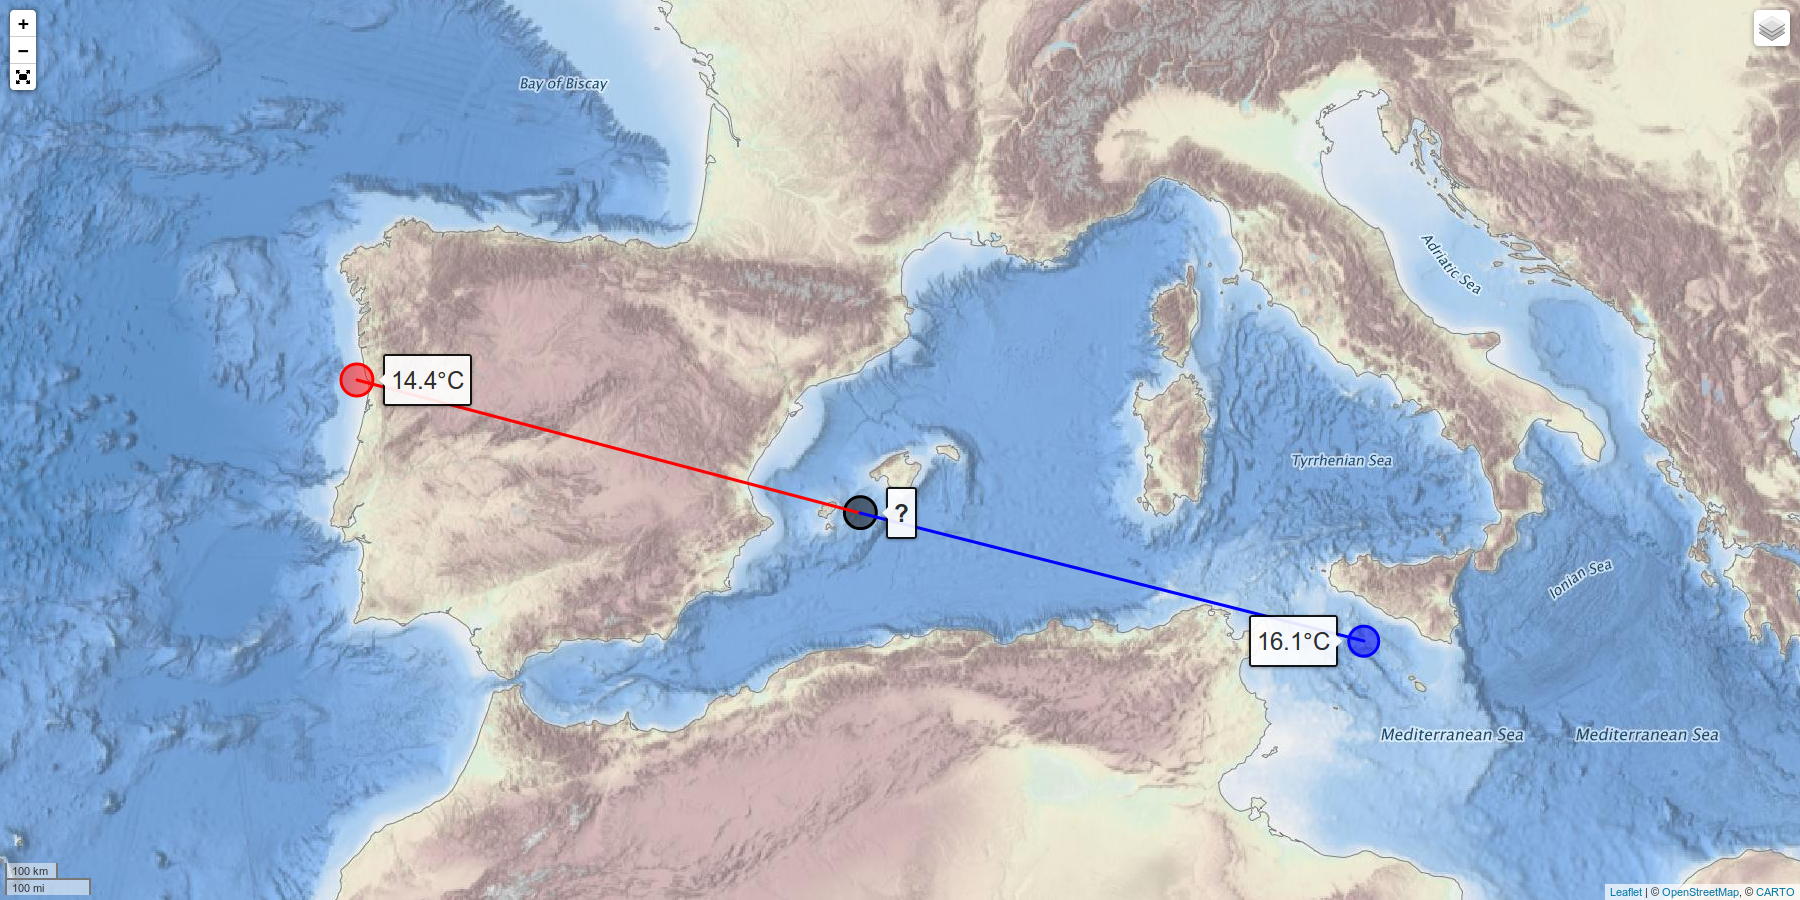
\includegraphics[width=\textwidth]{map_distance.png}
}
\end{frame}

%---------------------------------------------------------------------------------
\begin{frame}[c]
\frametitle{\mynum{6} A lot of processes taking place\ldots}

\Wider[2cm]{
\includegraphics[width=\textwidth]{ioio_0008s_0000_group3copy.jpg}
}
\end{frame}

%---------------------------------------------------------------------------------
\section{How do we do it?}
%---------------------------------------------------------------------------------

\begin{frame}
\frametitle{~}
\fontsize{30}{20}\selectfont How do we do it?
\end{frame}


\begin{frame}[b]
\frametitle{Data-Interpolating Variational Analysis}

\onslide*<1>{
Minimisation of a cost function taking into account:
\begin{enumerate}
\item Closeness to the observations
\item Regularity/smoothness of the solution
\end{enumerate}
\begin{eqnarray*}
{J}[\varphi]&=&\sum_{i=1}^{N}\mu_i \left[d_{i}-\varphi(x_{i},y_{i})\right]^{2} \label{eq:variab} \\
&+ &
 \int_{{D}}\left(
 {\boldsymbol{\nabla}}{\boldsymbol{\nabla}}\varphi : {\boldsymbol{\nabla}}{\boldsymbol{\nabla}}\varphi + { \alpha_{1}}
{\boldsymbol{\nabla}}\varphi \cdot {\boldsymbol{\nabla}}\varphi + \alpha_{0} \varphi^{2} \right) \mbox{d} {D},
\end{eqnarray*}
solved by a finite-element technique
\vfill
~
}

\onslide*<2->{
\faGithub~\url{https://github.com/gher-ulg/DIVA}\\ 
\aiDoi~\href{https://zenodo.org/record/836727}{\raisebox{-.25\height}{\includegraphics[height=.45cm]{figures/zenodo_diva}}}
\vspace{.25cm}
}

\Wider[2.cm]{
\includegraphics<2>[width=\textwidth]{map_base.png}
\includegraphics<3>[width=\textwidth]{map_contours.png}
\includegraphics<4>[width=\textwidth]{map_mesh.png}
\includegraphics<5>[width=\textwidth]{map_results.png}
}
\end{frame}


%---------------------------------------------------------------------------------
\begin{frame}[c]
\frametitle{DIVAnd: generalised, n-dimensional interpolation}

\onslide*<1>{
\begin{description}
\item[2013:] \raisebox{-.15cm}{\includegraphics[height=.6cm]{gnu-octave.png}} or MATLAB 
\item[2016:] \raisebox{-.15cm}{\includegraphics[height=.6cm]{Julia-languge}} \comment{faster, better, stronger}
\end{description}

\begin{figure}
\centering
\fbox{
\includegraphics[width=1.\textwidth]{sdc_divand}
}
\end{figure}

\vspace{.25cm}

\faFilePdfO~{\footnotesize \url{https://www.geosci-model-dev.net/7/225/2014/gmd-7-225-2014.pdf}}\\
\faGithub~{\footnotesize\url{https://github.com/gher-ulg/divand.jl}}
}

\onslide*<2>{
\Wider[1cm]{
\begin{eqnarray*}
  && K^{n,m}(r) \\  
  &=& c^{n,m} \frac{(2\pi)^{-\frac{n}{2}} }{2 (1-m)} r^{\frac{2-n}{2}}  \int_0^\infty {\mathrm J}_{\frac{n-2}{2}} (kr) k^{\frac{n-2}{2}} \frac{d}{dk} \left(  \frac{1}{(1+k^2)^{m-1}} \right) dk \nonumber  \\
&=&  c^{n,m} \frac{(2\pi)^{-\frac{n}{2}} }{2 (m-1)} r^{\frac{4-n}{2}}  \int_0^\infty {\mathrm J}_{\frac{n-4}{2}} (kr) k^{\frac{n-4}{2}}  \frac{k}{(1+k^2)^{m-1}}  dk  \label{eqn:Kp_recursion_step1} \\
 \label{eqn:Kp_recursion}
&=&  \frac{1}{4 \pi (m-1)} \frac{c^{n,m}}{c^{n-2,m-1}} K^{n-2,m-1}(r)
\end{eqnarray*}
}

\parbox{1.5cm}{
where
}\parbox{9cm}{
\begin{itemize}
\item[] $n$ is the dimension
\item[] $m$ is the highest derivative 
\item[] $K^{n,m}$ is the Kernel 
\item[] $J_{\nu}(r)$ is the Bessel function of first kind or order $\nu$
\end{itemize}
}
}

\end{frame}

%---------------------------------------------------------------------------------

\begin{frame}
\frametitle{~}
\footnotesize
\begin{table}[c]
\centering
\begin{tabular}{R{5.5cm}|L{5.5cm}}
\textcolor{bluesdn}{Problem}			& \textcolor{bluesdn}{Solution in DIVA}		\\
										& 												\\
\mynum{1} Synopticity error 			& \textcolor{gray}{Regularity constrain in cost function}		\\
\mynum{2} Representativeness error		& 												\\
										& 												\\
\mynum{3} Many observations			& Numerical cost (almost) independent on the number of data points\\
										& 												\\
\mynum{4} Interpolate at many locations	& \textcolor{gray}{Finite-element solver}	\\
										& 												\\
\mynum{5} Anisotropy					& Finite-element solver							\\ 
										& 												\\
\mynum{6} Currents 						& \textcolor{gray}{Advection included in the cost function}		\\


\end{tabular}
\end{table}
\end{frame}

%---------------------------------------------------------------------------------
\begin{frame}[t]
\frametitle{Notebooks: user-interface}

\begin{enumerate}
\item Documentation, including equations and export to pdf
\item Code fragments for different steps of the interpolation
\item Figures illustrating the data or intermediate results
\end{enumerate}

\onslide*<1>{
\begin{figure}
\centering
\includegraphics[width=.8\textwidth]{notebook_ex}
\end{figure}
}

\end{frame}

\begin{frame}[c]
\frametitle{Notebooks: workflow description}

\onslide*<1>{

\fbox{
\includegraphics[width=\textwidth]{nature_notebooks}
}
\vspace{.5cm}

\url{http://www.nature.com/news/interactive-notebooks-sharing-the-code-1.16261}

}

\onslide*<2>{Provide the jupyter-notebooks\\ 
along with the data product (interpolation)\\

\begin{description}
\item[Easy to share:] \url{http://nbviewer.jupyter.org/}, \url{http://github.com/}\\
\item[Make easier] the \textbf{reproducibility} and peer-review
\end{description}

}


\end{frame}
%---------------------------------------------------------------------------------

\section{Why do we need a VRE?}

\begin{frame}
\frametitle{~}

\fontsize{30}{20}\selectfont Why do we need\\
\mynum{V}irtual \\
\mynum{R}esearch \\
\mynum{E}nvironments?
\end{frame}

%---------------------------------------------------------------------------------
\begin{frame}
\frametitle{Computational resources}

Storage and inversion of huge matrices

\vspace{1cm}

\textbf{Typical case:} \\
\begin{description}
\item[Horizontal grid:] 500 $\times$ 500
\item[Vertical levels:] 50 depth levels
\item[Time periods:] 20 
\end{description}


\end{frame}


%---------------------------------------------------------------------------------
\begin{frame}[c]
\frametitle{Better access to SeaDataCloud data and tools}

People connect, access the data, and work!

\vspace{.5cm}

\begin{figure}
\centering
\includegraphics[width=\textwidth]{SDC_software}
\end{figure}


\end{frame}
%---------------------------------------------------------------------------------
\begin{frame}
\frametitle{Installed/deployed once, used many times}

\includegraphics[height=.6\textwidth]{CartelDIVA}~\includegraphics[height=.6\textwidth]{Calvi07_033logo.jpg}

Installing is sometimes much harder than running the code\ldots 

\end{frame}
%---------------------------------------------------------------------------------

%Big Data? check the 3 V's
%Volume: it's big but not huge
%Velocity: yes, the dataset is increasing fast
%Variety: definitively

\begin{frame}[t]
\frametitle{DIVAnd in the VRE with jupyterhub}

\parbox{2cm}{
\includegraphics[width=1.75cm]{logo_hub}
}\parbox{8cm}{Management of multiple instances\\ of the single-user Jupyter notebook server}

\begin{figure}
\includegraphics[width=\textwidth]{jupyterhub_ex}
\end{figure}

\faGithub~\url{https://github.com/jupyterhub/jupyterhub}

Demo available at \url{https://hub-test.oceanbrowser.net/}\\ (deployed at CINECA via Docker)

\end{frame}
%---------------------------------------------------------------------------------

%\begin{frame}
%\frametitle{Orchestration methods}
%
%\begin{description}
%\item[Kubernetes] (\url{https://github.com/jupyterhub/kubespawner})\\
%{\footnotesize Kubernetes = open-source system for automating deployment, scaling, and management of containerized applications}\\
%\textbf{+}\quad  developed by jupyterhub
%\item[Docker swarm] (\url{https://docs.docker.com/engine/swarm/})\\
%{\footnotesize Swarm = cluster of Docker Engines\\
%Current versions of Docker include swarm mode for natively managing a swarm} \\
%\textbf{+}\quad integrated with Docker Engine
%\end{description}
%
%\end{frame}
%%---------------------------------------------------------------------------------

\begin{frame}
\frametitle{I/O}
\begin{tabular}{R{7cm}C{3cm}}
\textbf{Authentication} & MarineID or \raisebox{-.35cm}{\includegraphics[height=1.25cm]{b2access}}\\
\textbf{Inputs:} CDI data and user data & \raisebox{-.35cm}{\includegraphics[height=1.25cm]{b2drop}}\\
\textbf{Results} of the interpolation  & \raisebox{-.35cm}{\includegraphics[height=1.25cm]{b2drop}~\includegraphics[height=1.25cm]{b2safe}}\\
\textbf{Outputs:} data products, climatologies, gridded fields & \raisebox{-.5cm}{\includegraphics[height=1.25cm]{b2safe}}
\end{tabular}
\end{frame}
%---------------------------------------------------------------------------------
\section{Conclusion}

\begin{frame}
\frametitle{Summary}
\begin{itemize}
\item<1->[\Checkmark] Spatial interpolation is a \textbf{frequent}\\ but \textbf{not trivial} operation in ocean sciences
\item<2->[\Checkmark] \textbf{Specific} tools (DIVA, DIVAnd)\\ have been designed for data interpolation
\item<3->[\Checkmark] With a VRE, \textbf{more} users can access\\ \textbf{more} easily SeaDataCloud resources\\ (metadata, data \& tools)
\end{itemize}
\end{frame}

%---------------------------------------------------------------------------------


\begin{frame}
\frametitle{Thanks for your attention}
\begin{table}[c]
\centering
\begin{tabular}{R{4cm}|L{4cm}}
Tools 					& \href{http://leafletjs.com/}{Leaflet}							\\
						& \href{https://github.com/gher-ulg/DIVA}{DIVA}					\\
						& \href{https://github.com/gher-ulg/divand.jl}	{DIVAnd}			\\
						& \\
Map layers 				& \href{http://www.emodnet-bathymetry.eu/}{EMODnet Bathymetry}	\\
						& \href{https://earthdata.nasa.gov}{Earth At Night 2012}			\\	
						& \\				
MedSea observations		& \href{http://sextant.ifremer.fr/record/cd552057-b604-4004-b838-a4f73cc98fcf/}{Temperature and salinity observation collection V1.1}\\


\end{tabular}
\end{table}
\end{frame}

\begin{frame}[b]
\frametitle{The temperature at the "?"}

\Wider[2cm]{
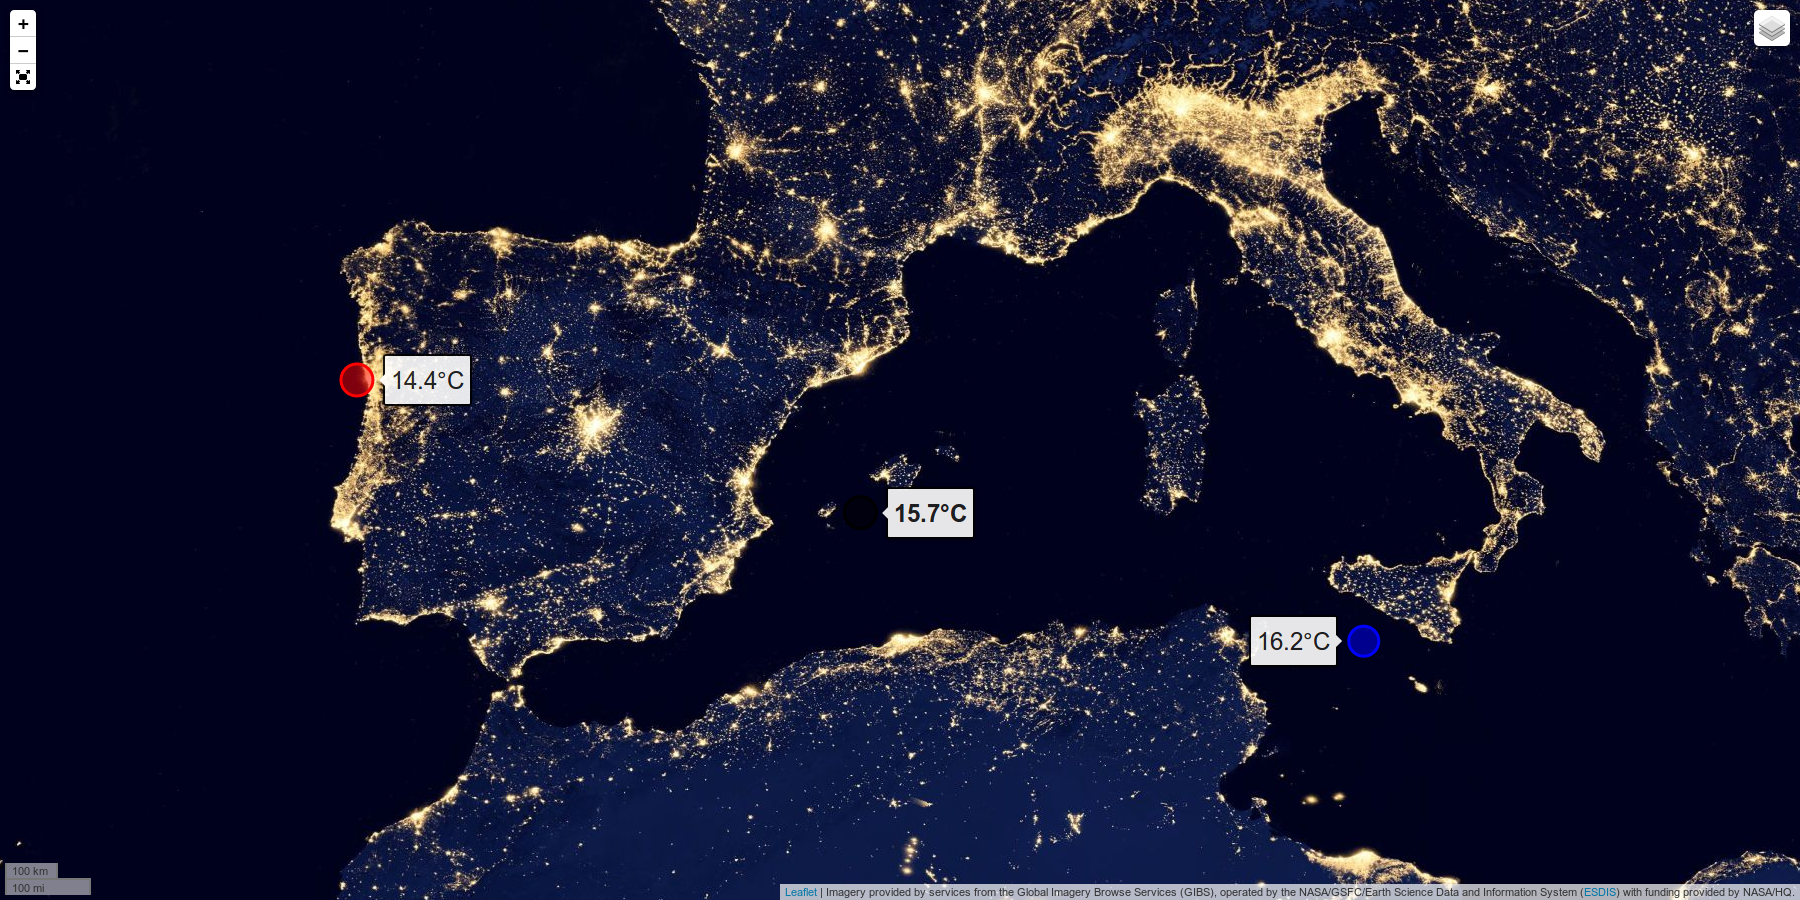
\includegraphics[width=\textwidth]{map_conclusion.png}
}


\end{frame}


\end{document}
